\section{Evaluation}

\subsection{Implementation of Transfer Learning}
In our first implementation, as shown on figure \ref {fig:xceptiona}, we feed an image to Xception model and took the average pooling of the last layer from Xception, and then we used a classification layer directly to classify the image. We used the cross-entropy loss for training. For this approach, we experimented by freezing the weights from Xception and by training it from scratch. 

\begin{figure}[h]
 \centering
  \begin{subfigure}[b]{\linewidth}
 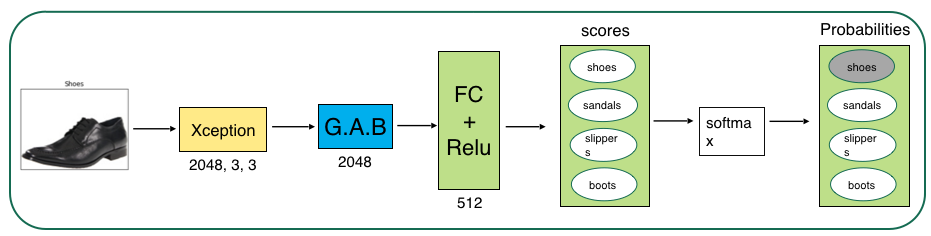
\includegraphics[width=\linewidth]{figs/xception_1.png}
  \caption{Version 1}
  \label{fig:xceptiona}
  \end{subfigure}
    \hfill
  \begin{subfigure}[b]{\linewidth}
 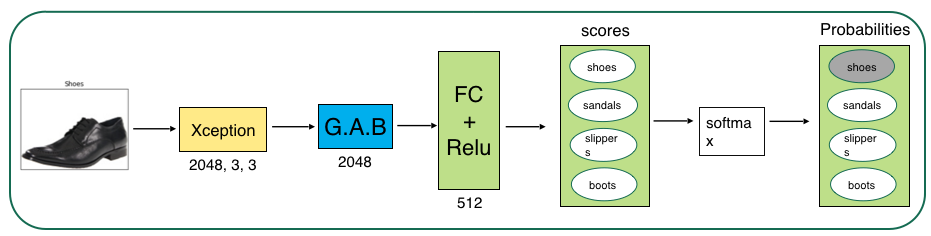
\includegraphics[width=\linewidth]{figs/xception_1.png}
 \caption{Version 2}
  \label{fig:xceptionb}
  \end{subfigure}
    \hfill    
 \caption{Implemented transfer learning architectures.}
 \label{fig:xception}
\end{figure}

On the second implementation, as shown on figure \ref{fig:xceptionb}, we froze learned weights from Xception but we added a fully connected layer before the prediction layer. For this fully connected, We used 512 Victor dimension because we wanted to match it with the best embedding size of our implementation for siamese network for the comparison. 

We used Adam optimizer with learning rate of 0.001 for all transfer learning approaches.

\subsection{Implementation of Siamese Network}

The architecture of our implementations of the siamese network is shown as figure \ref{fig:model}. Our network consists of a batch input layer and a deep CNN followed by L2 normalization, which results in the image embedding. This is followed by a loss function during training. Note that the siamese network was designed originally for calculating the similarity between images, not the image classification. Normally, it would have a distance function to compute the similarity between the two embedding vectors as the final outputs. However, our project is for the image classification problem, so we add one more fully connected layer on top of that and trained it to predict the class of the embeddings (instead of the image). 

\begin{figure}[h]
  \centering
  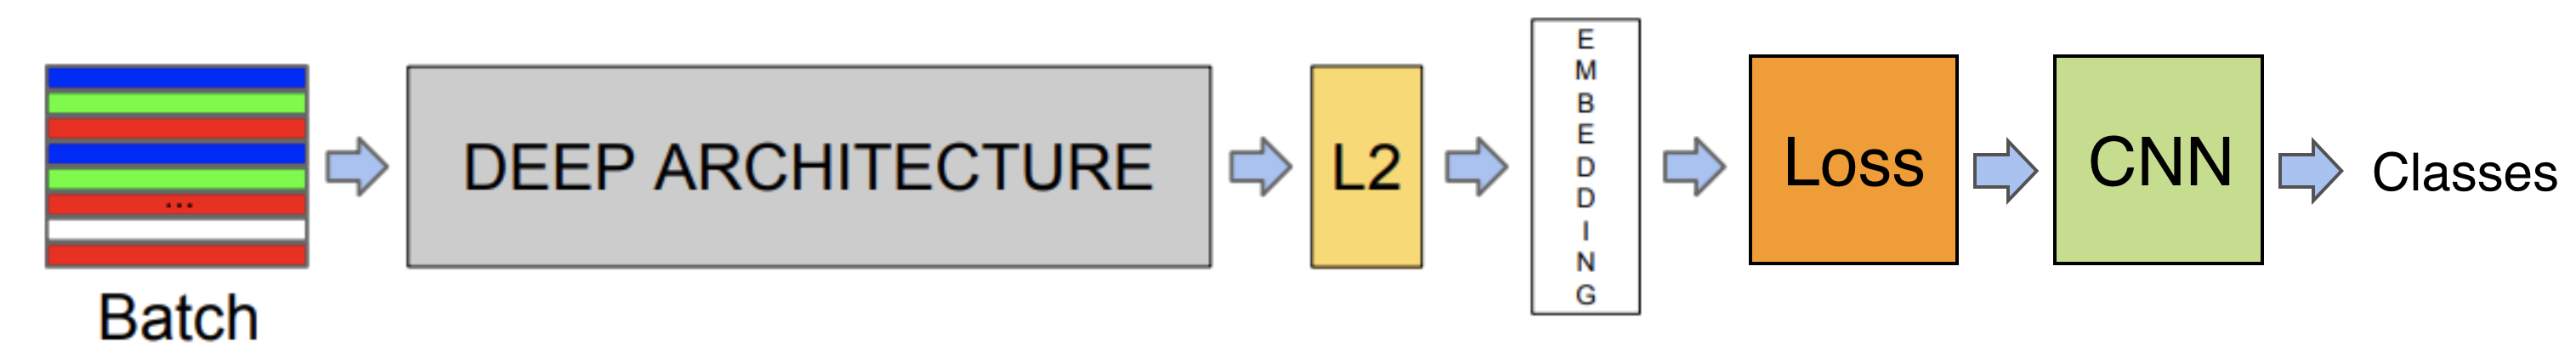
\includegraphics[width=\linewidth]{figs/model.png}
  \caption{The architecture of our model.}
  \label{fig:model}
\end{figure}

In this project, we implemented three variants of the siamese network. The first one is with contrastive loss, and the second one is with triplet loss. The third one is the combination of transfer learning and the one with triplet loss.

For the implementation of contrastive loss, we build the model and implement the loss function by ourselves using Keras and Tensorflow. The implementation can be partitioned into three steps: 1) generating image pairs, 2) construct the architecture of the siamese neural network, 3) using contrastive loss to train the model. We adopt a simple strategy to make the image pairs. The positive sample is picked randomly from the same category as the anchor, and label with 1. On the other hand, we grab the negative sample randomly from classes that are different from the anchor and label it with 0. Figure \ref{fig:pairs} shows the examples of the positive and negative pairs. 

\begin{figure}[h]
  \centering
  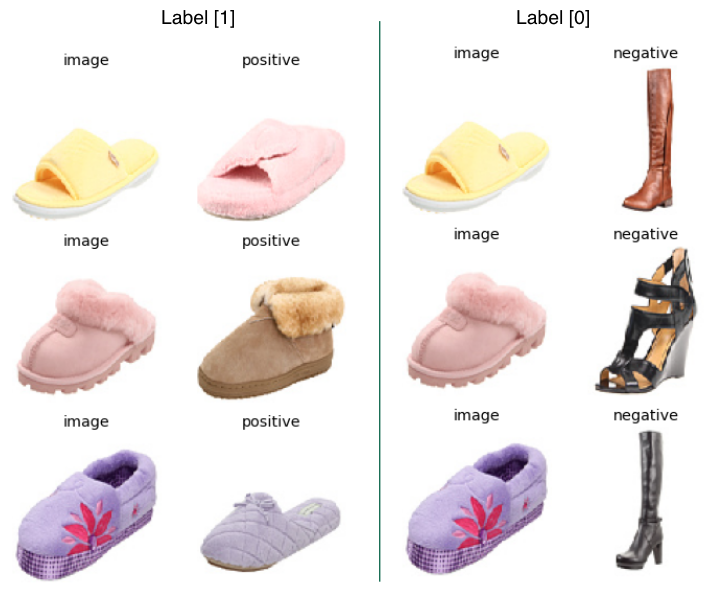
\includegraphics[width=0.9\linewidth]{figs/pairs.png}
  \caption{Examples of the positive and negative pairs.}
  \label{fig:pairs}
\end{figure}

For the implementation of triplet loss, we implement it by calling the TripletSemiHardLoss function in TensorFlow Addons. As shown in the paper \cite{schroff2015facenet}, the best results are from Semi-Hard triplets. This implementation contains three steps that are similar to the contrastive loss one. And we used the same strategy to make the triplets. The only difference is that we use the offline mining approach for the first implementation, while the online mining approach for the second one. Offline mining means that pairs are defined at the beginning of the training. Online mining means that triplets are defined for every batch during the training. And the latter one has been proved in better training efficiency and performance.

The CNN model in our implementations is represented in figure \ref{fig:cnn}. The hidden layers consist of convolutional layers, pooling layers, fully connected layers, and normalization layers (ReLU). All the parameters we used for training are as shown in the figure.  

\begin{figure}[h]
 \centering
 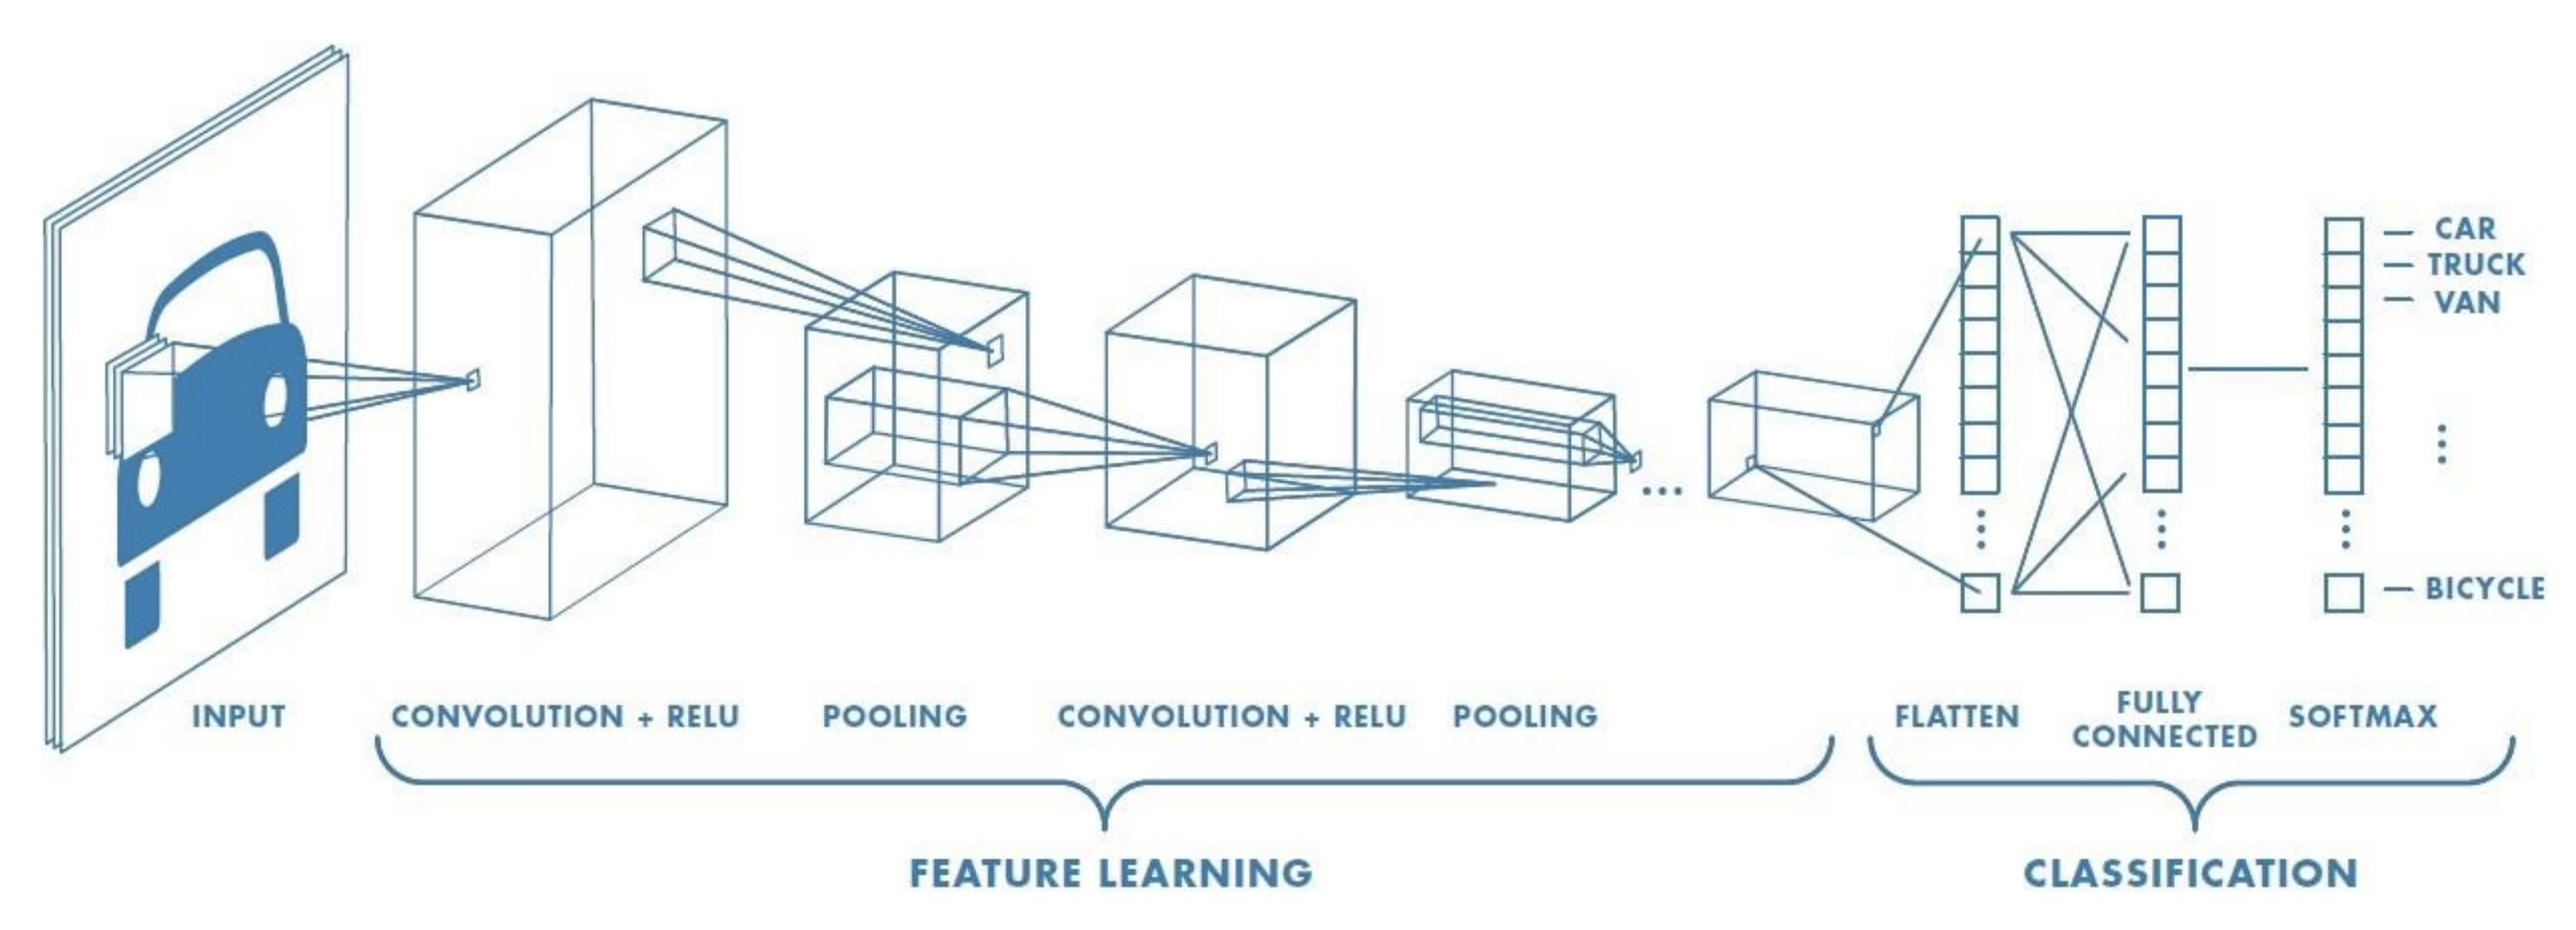
\includegraphics[width=\linewidth]{figs/cnn.png}
 \caption{The Convolutional Neural Network (CNN) in our implementations.}
 \label{fig:cnn}
\end{figure}

Furthermore, to improve the performance of the siamese network, we implemented another version with transfer learning. As shown in the figure, we used the Xception to extract the features firstly, followed by a global average pooling layer, and applied two dense layers on top of that. And this model is trained with the triplet loss. The implementation details are showed in figure \ref{fig:xception_cnn}. 

We used Adam optimizer with learning rate of 0.001 for all Siamese Network approaches. 

\begin{figure}[h]
  \centering
  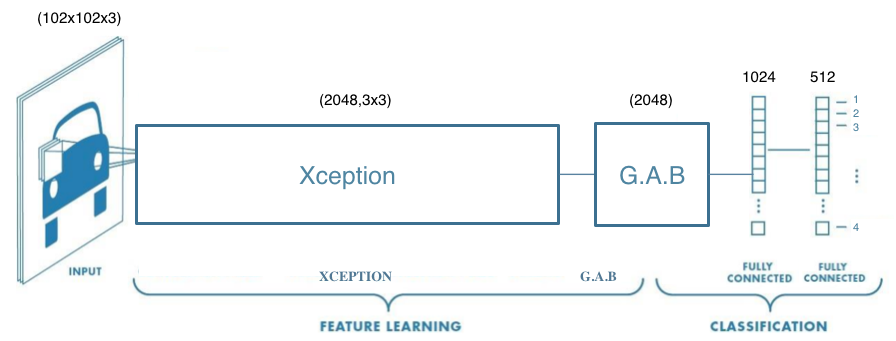
\includegraphics[width=\linewidth]{figs/xception_cnn.png}
  \caption{Applying  Xcepetion into our implementation.}
  \label{fig:xception_cnn}
\end{figure}

\subsection{Results and Analysis}
Table \ref{table:resultA} summaries the results of our experiment. T0 is the a accuracy for directly classifying the features extracted from Xception. T1 is the result of adding a single fully connected layer before the prediction. This lead to 1\% decrease of accuracy. Most likely the large dense vector lead to over-fitting. We also trained Xception from scratch on this data set as shown in T2, and this improved the results by around 4\%. The next 3 lines are the result siamese network implementation. S0 and S1 are the results for the same model but with a different loss function. In theory and as discussed in the original paper, triplets of training data samples would outperform contrastive loss. However, it is not the case in our experiment. Using contrastive loss results in 1.5\% better accuracy. Finally, the idea where we uses the features from transfer learning and add to dense layers with the siamese network idea of triplets did improve the features for classification. As we see in the last row, the accuracy improved more than 4\% from just applying transfer learning and it did slightly outperform training Xception from scratch by .7\%. This improvement can also be visualized in figure \ref{fig:2Dprojection}. It is a visualization of the embedded test data projected to 2D space with UMAP using Projector from tensorflow. It is clear that the features are much improved and can easily be classified compared with the exception model trained from scratch.

\begin{table}[ht]
    \caption{Summary of the results on 1500 images per category} 
    \centering 
    \begin{tabular}{c c c c} 
    \hline\hline 
    
    model & Accuracy \% & Epochs & Time (mins)  \\% inserts table
    \hline % inserts single horizontal line
    Xception (T0) & 91.8 & 20 & 1.8 \\% inserting body of the table
    Xception+dense (T1) & 90.7 & 20 & 3.5 \\% inserting body of the table
    Xception All (T2) & 95.1 & 10 & 5.4 \\% inserting body of the table
    Our Siamese+Con. Loss (S0) & 92.57 & 32 & 6 \\% inserting body of the table
    Our Siamese+Triplet. Loss (S1) & 91.02  & 20& 2 \\% inserting body of the table
    Xception+Siamese (S2) & 95.85 & 10 & 2 \\% inserting body of the table
    \hline 
    \end{tabular}
\label{table:resultA} % is used to refer this table in the text
\end{table}

\begin{table}[ht]
    \caption{Summary of the results on 2500 images per category} 
    \centering 
    \begin{tabular}{c c c c} 
    \hline\hline 
    
    model & Accuracy \% & Epochs & Time (mins)  \\% inserts table
    \hline % inserts single horizontal line
    Xception (T0) & 89.9 & 20 & 4 \\% inserting body of the table
    Xception+dense (T1) & 89.3 & 20 & 4 \\% inserting body of the table
    Xception All (T2) & 94.0 & 10 & 6 \\% inserting body of the table
    Our Siamese+Con. Loss (S0) & 90.2 & 32 & 14 \\% inserting body of the table
    Our Siamese+Triplet. Loss (S1) & - & - & - \\% inserting body of the table
    Xception+Siamese (S2) & - & - & - \\% inserting body of the table
    \hline 
    \end{tabular}
\label{table:resultB} % is used to refer this table in the text
\end{table}

The result summary on table \ref{table:resultB} is for a larger data set where we used 2500 from each class. However, we had to do some data augmentation (mirror only) for the slippers class since it is only 1283 images. This decreased the accuracy in all experiments. We believe that it is because all the images are pictured in the same orientation. So, using mirrored orientated images for a single class confused the models. This confusion affected all the classes not just the slippers class as shown on figure \ref{fig:sia_con_data}.



%\begin{figure}[h]
 % \centering
 %  \begin{subfigure}[b]{0.48\linewidth}
 %  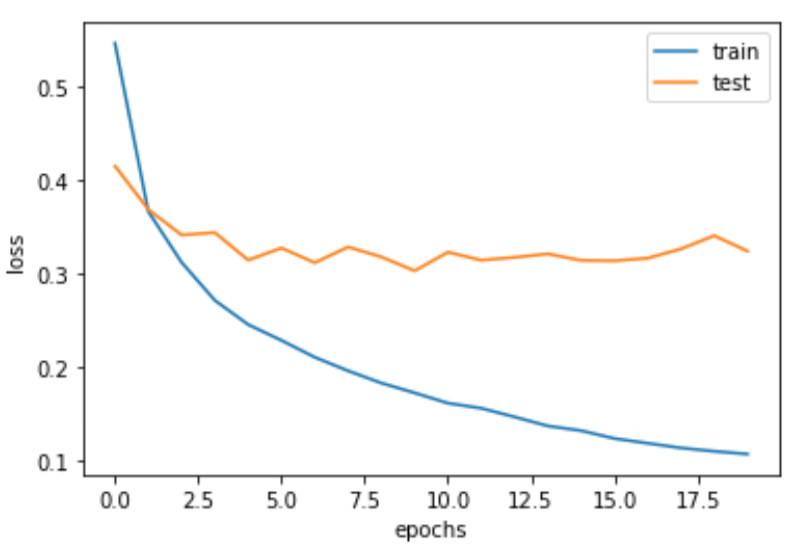
\includegraphics[width=\linewidth]{figs/transfer_loss.png}
 %  \caption{Transfer Learning version 1}
 %  \label{fig:con_loss}
 %  \end{subfigure}
 %  \hfill
 %   \begin{subfigure}[b]{0.48\linewidth}
 %   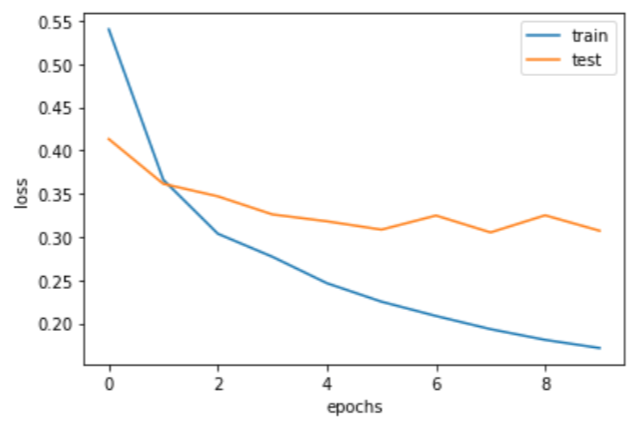
\includegraphics[width=\linewidth]{figs/transfer_loss_2.png}
 %   \caption{Transfer Learning version 2}
 %   \label{fig:tri_loss}
 %  \end{subfigure}
 %    \hfill
   %  \begin{subfigure}[b]{0.48\linewidth}
  %  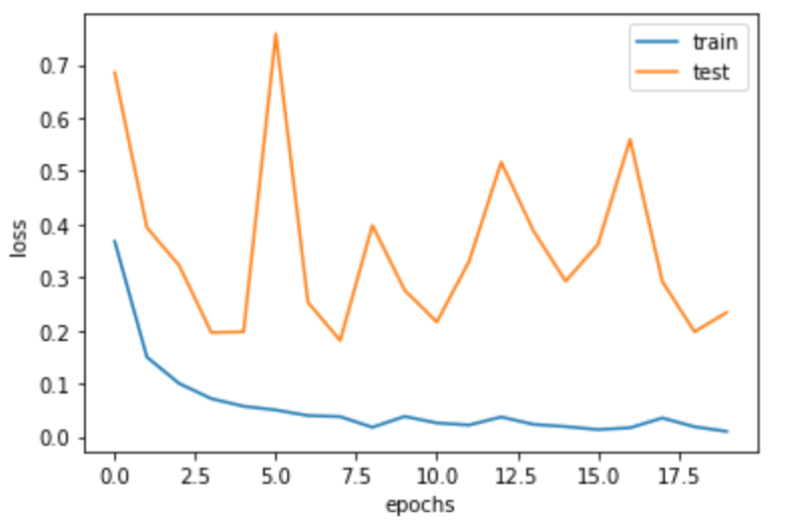
\includegraphics[width=\linewidth]{figs/transfer_loss_3.png}
  %  \caption{Transfer Learning version 3}
 %   \label{fig:tri_loss_2}
 %  \end{subfigure}
 %  \hfill
 %    \caption{Training loss of the three implementations of transfer Learning.}
 %    \label{fig:tertrainloss}
 %\end{figure}


 %\begin{figure}[h]
 %  \centering
 %  \begin{subfigure}[b]{0.48\linewidth}
 %  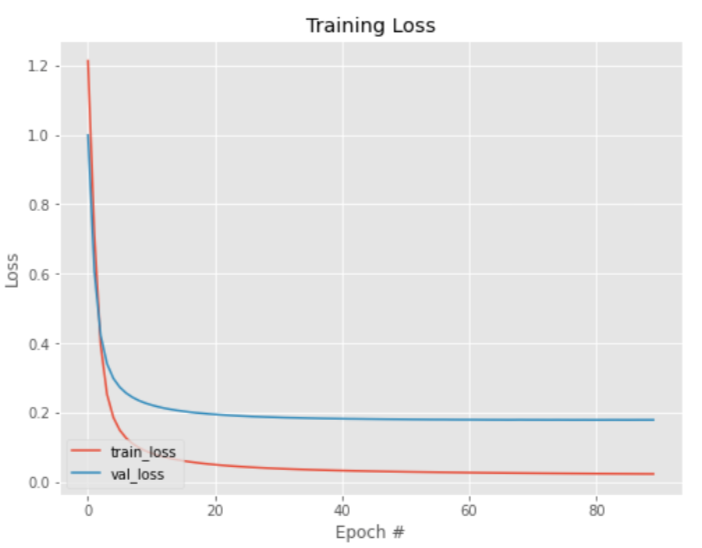
\includegraphics[width=\linewidth]{figs/con_loss.png}
 %  \caption{Contrastive loss}
  % \label{fig:con_loss}
  % \end{subfigure}
  % \hfill
 %   \begin{subfigure}[b]{0.48\linewidth}
  %  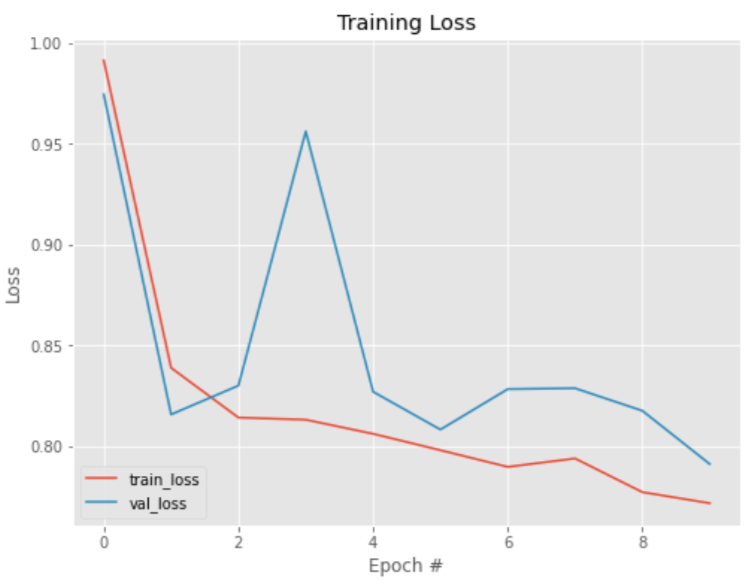
\includegraphics[width=\linewidth]{figs/tri_loss.png}
 %   \caption{Triplet loss}
 %   \label{fig:tri_loss}
 %  \end{subfigure}
 %    \hfill
 %    \begin{subfigure}[b]{0.48\linewidth}
 %   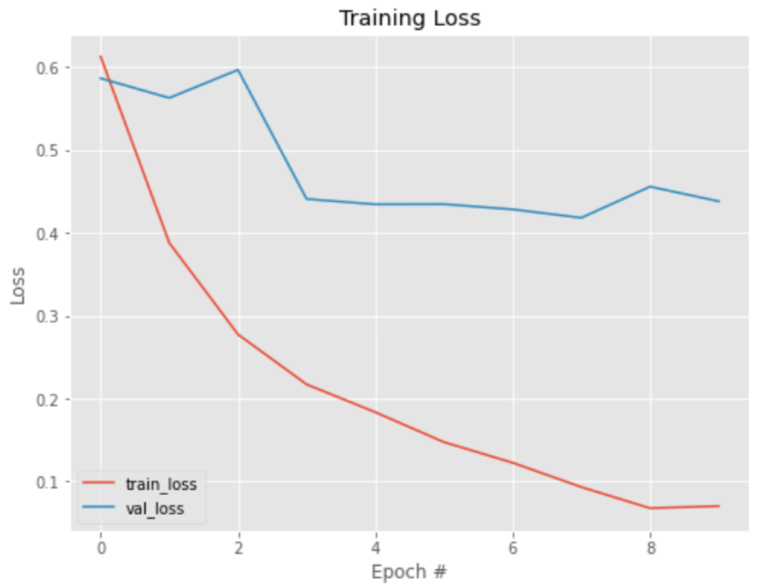
\includegraphics[width=\linewidth]{figs/tri_loss_2.png}
  %  \caption{Transfer Learning and triplet loss}
 %   \label{fig:tri_loss_2}
 %  \end{subfigure}
  % \hfill
  %   \caption{Training loss of the three implementations of the siamese network.}
 %    \label{fig:siatrainloss}
 %\end{figure}
 
 \begin{figure}[h]
  \centering
  \begin{subfigure}[b]{\linewidth}
  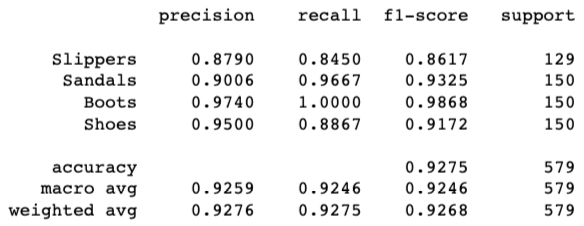
\includegraphics[width=\linewidth]{figs/sia_con_data1.png}
  \caption{Results with the dataset 1.}
  \label{fig:sia_con_data1}
  \end{subfigure}
  \hfill
   \begin{subfigure}[b]{\linewidth}
   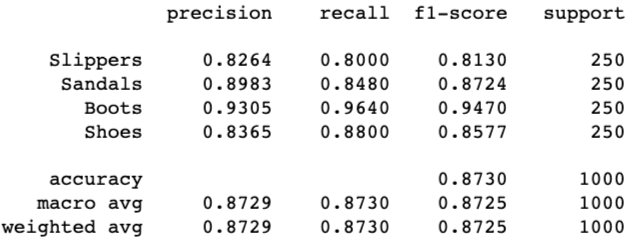
\includegraphics[width=\linewidth]{figs/sia_con_data2.png}
   \caption{Results with the dataset 2.}
   \label{fig:sia_con_data2}
  \end{subfigure}
    \hfill
    \caption{Comparison of the results of the siamese network implementation with contrastive loss with two datasets.}
    \label{fig:sia_con_data}
\end{figure}

\begin{figure}[h]
  \centering
  \begin{subfigure}[b]{0.48\linewidth}
  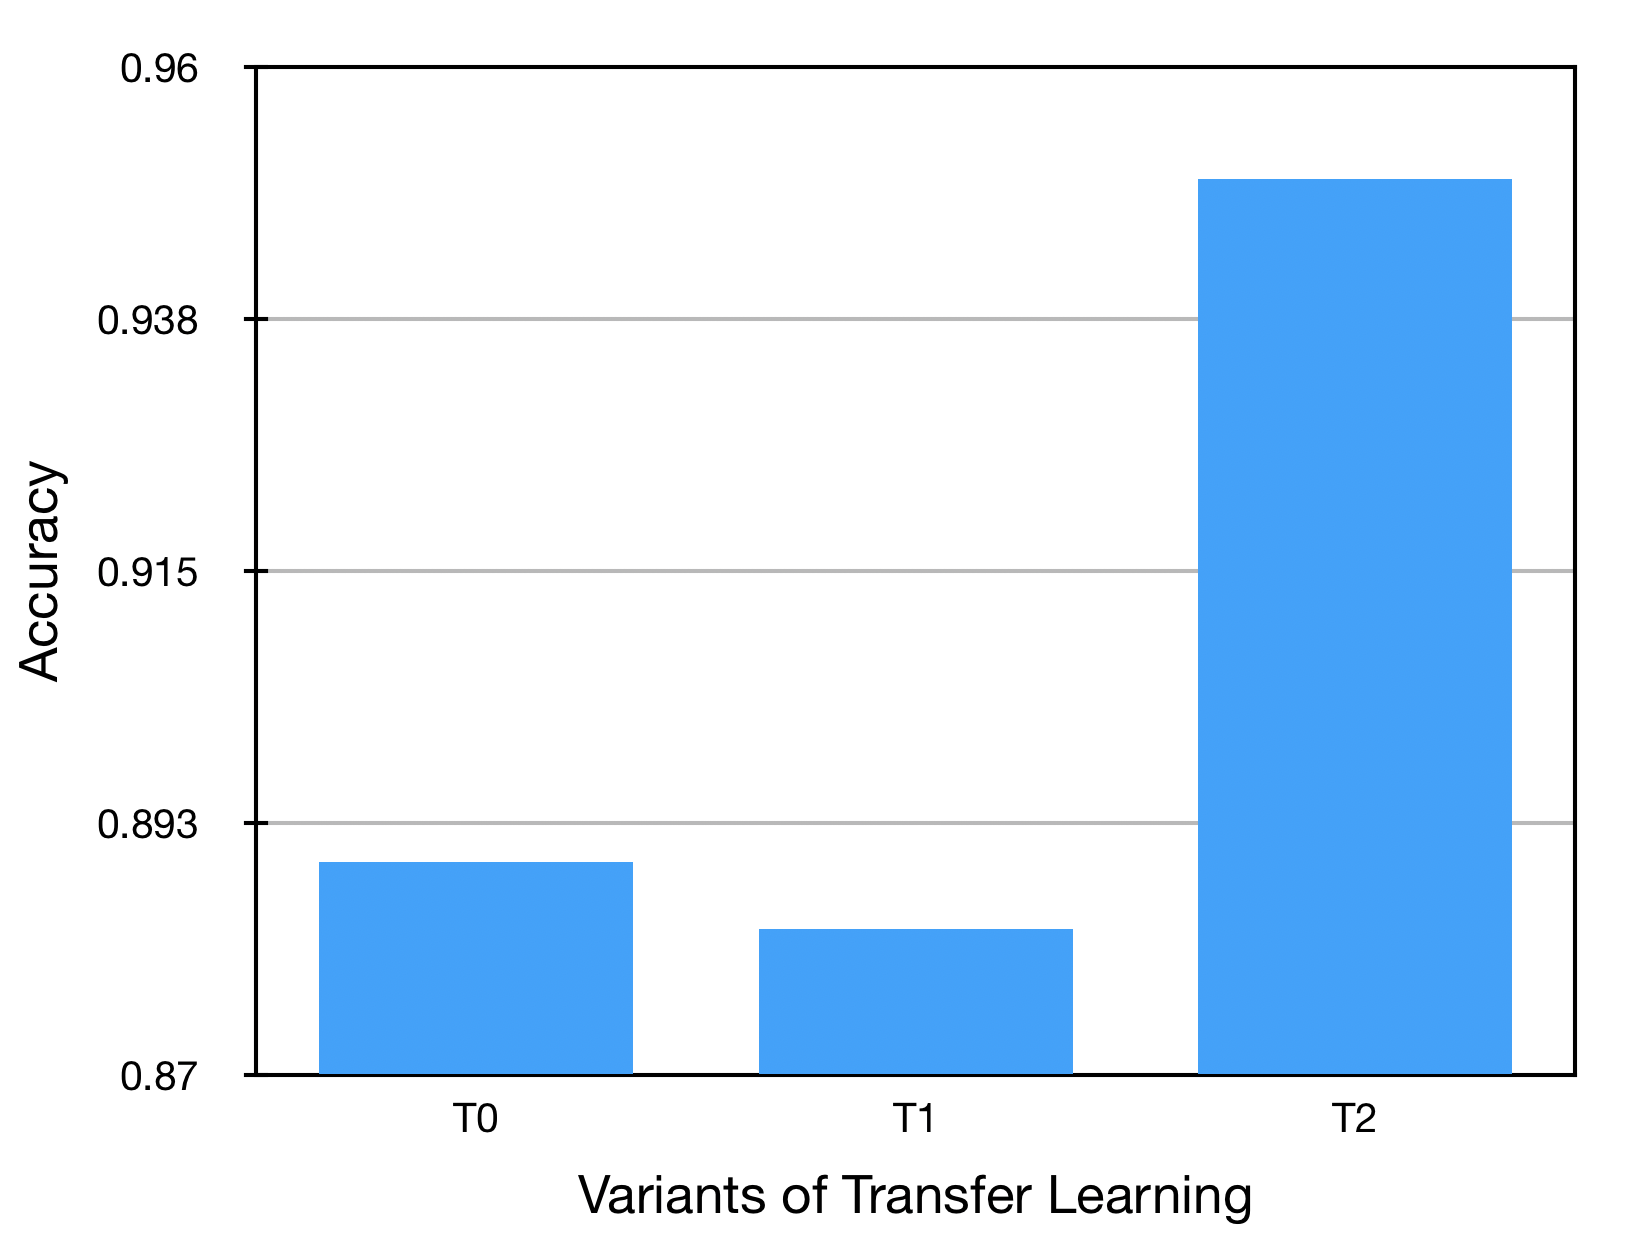
\includegraphics[width=\linewidth]{figs/acc_ter.png}
  \caption{Accuracy comparison}
  \label{fig:con_loss}
  \end{subfigure}
  \hfill
   \begin{subfigure}[b]{0.48\linewidth}
   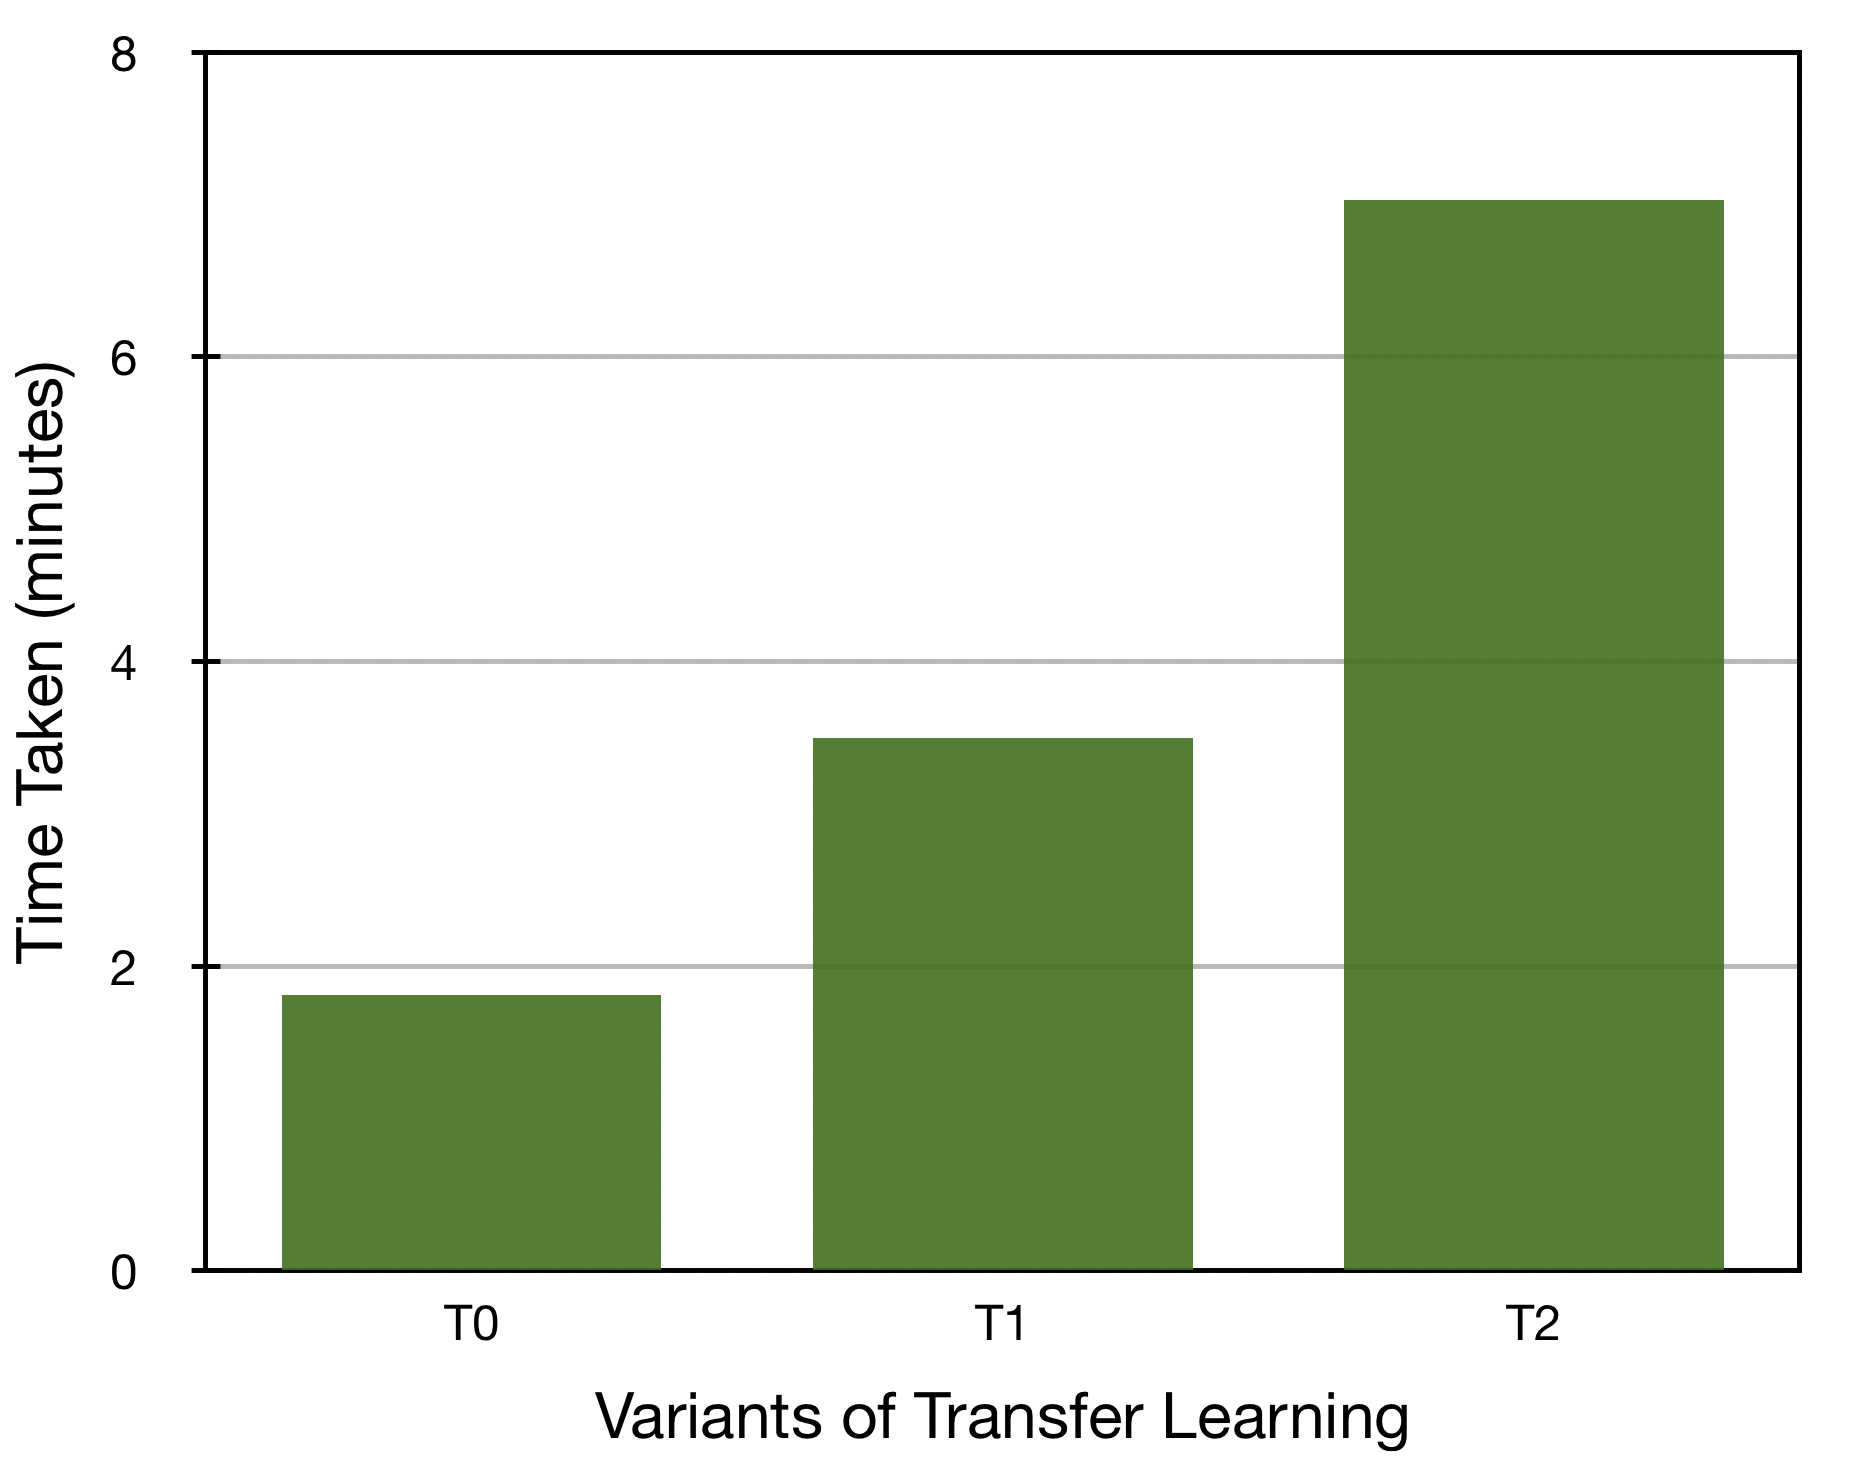
\includegraphics[width=\linewidth]{figs/time_ter.png}
   \caption{Time taken comparison}
   \label{fig:tri_loss}
  \end{subfigure}
    \hfill
    \caption{Comparison of the three implementations of the transfer learning.}
    \label{fig:siatrainloss1}
\end{figure}

\begin{figure}[h]
  \centering
  \begin{subfigure}[b]{0.48\linewidth}
  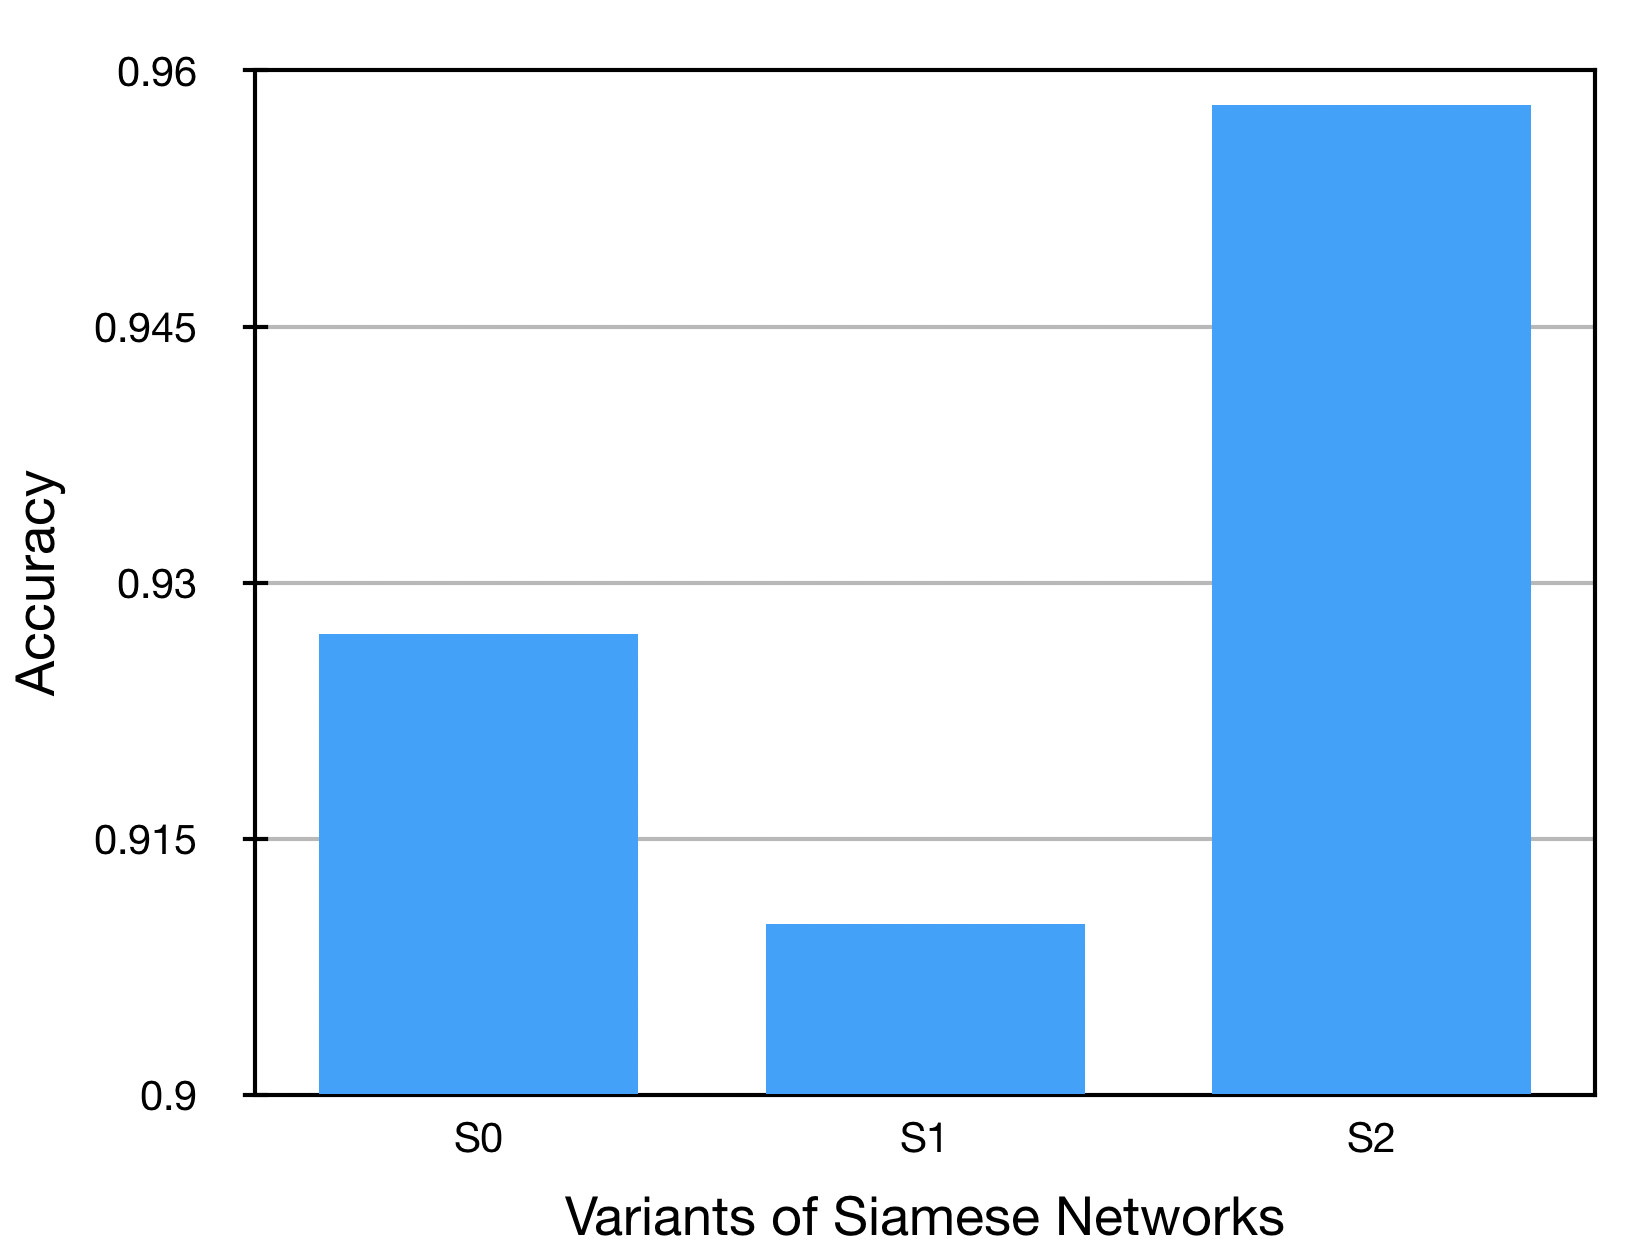
\includegraphics[width=\linewidth]{figs/acc_sia.png}
  \caption{Accuracy comparison}
  \label{fig:con_loss}
  \end{subfigure}
  \hfill
   \begin{subfigure}[b]{0.48\linewidth}
   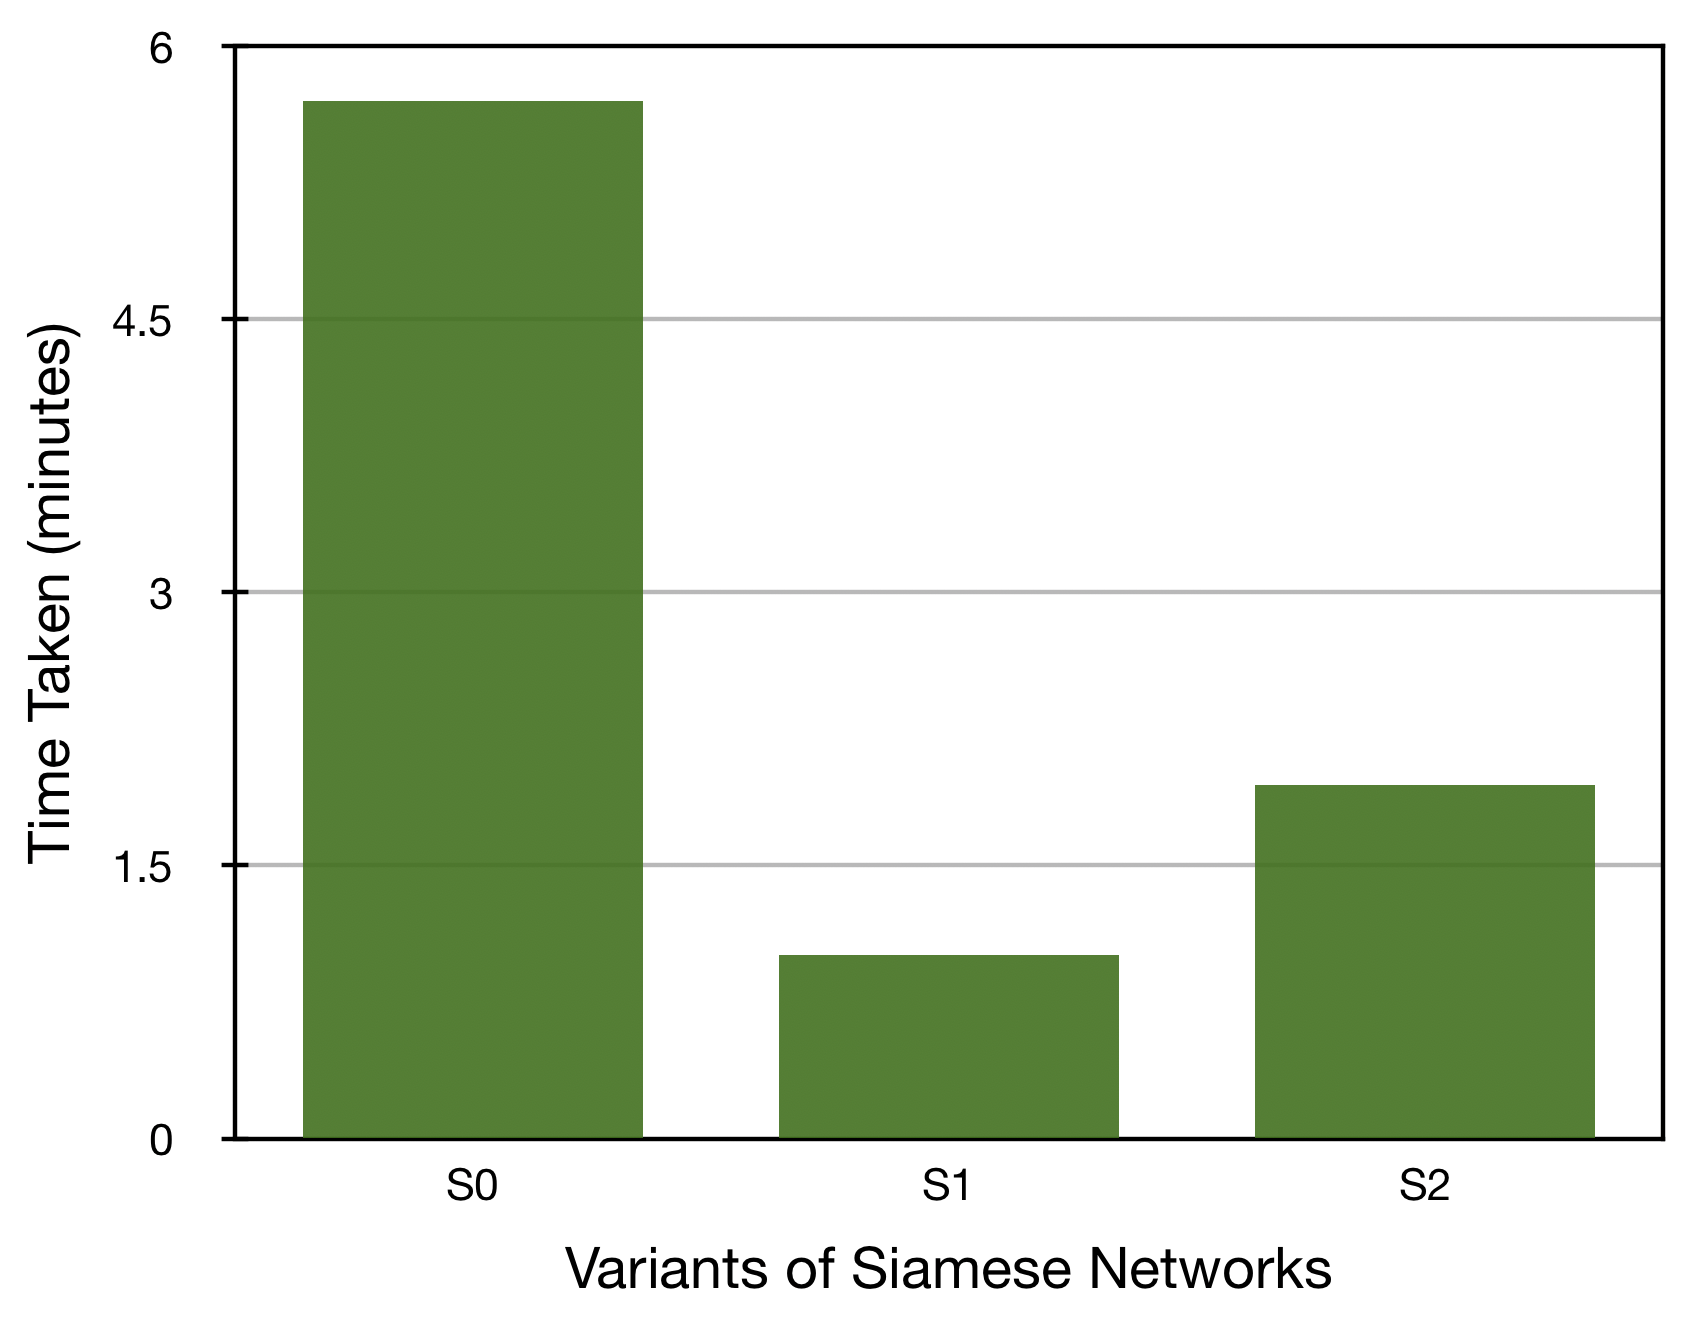
\includegraphics[width=\linewidth]{figs/time_sia.png}
   \caption{Time taken comparison}
   \label{fig:tri_loss}
  \end{subfigure}
    \hfill
    \caption{Comparison of the three implementations of the siamese network.}
    \label{fig:siatrainloss2}
\end{figure}


\begin{figure}[h]
  \centering
  \begin{subfigure}[b]{0.48\linewidth}
  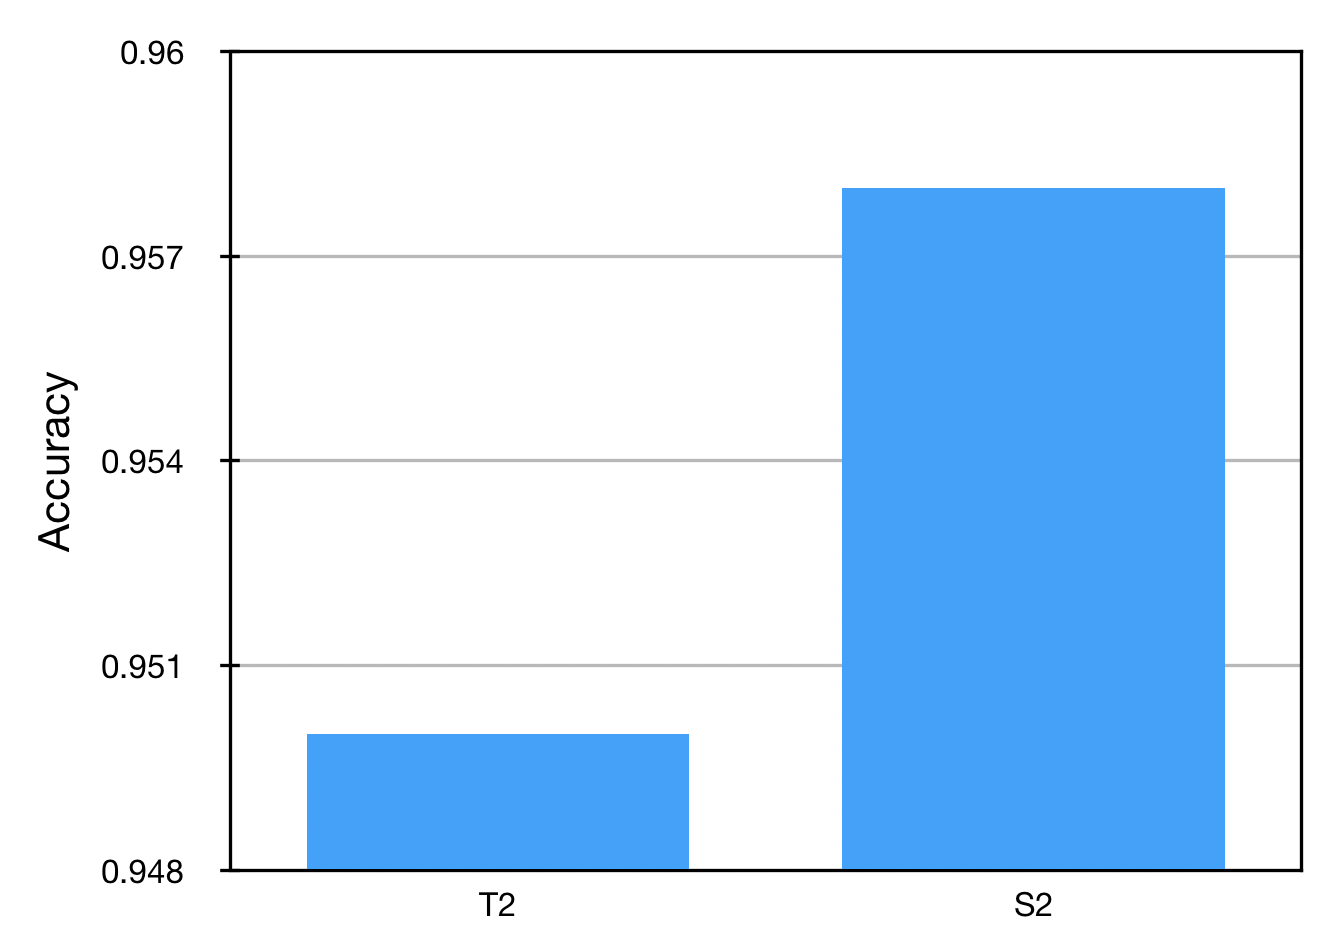
\includegraphics[width=\linewidth]{figs/acc.png}
  \caption{Accuracy comparison}
  \label{fig:con_loss}
  \end{subfigure}
  \hfill
   \begin{subfigure}[b]{0.48\linewidth}
   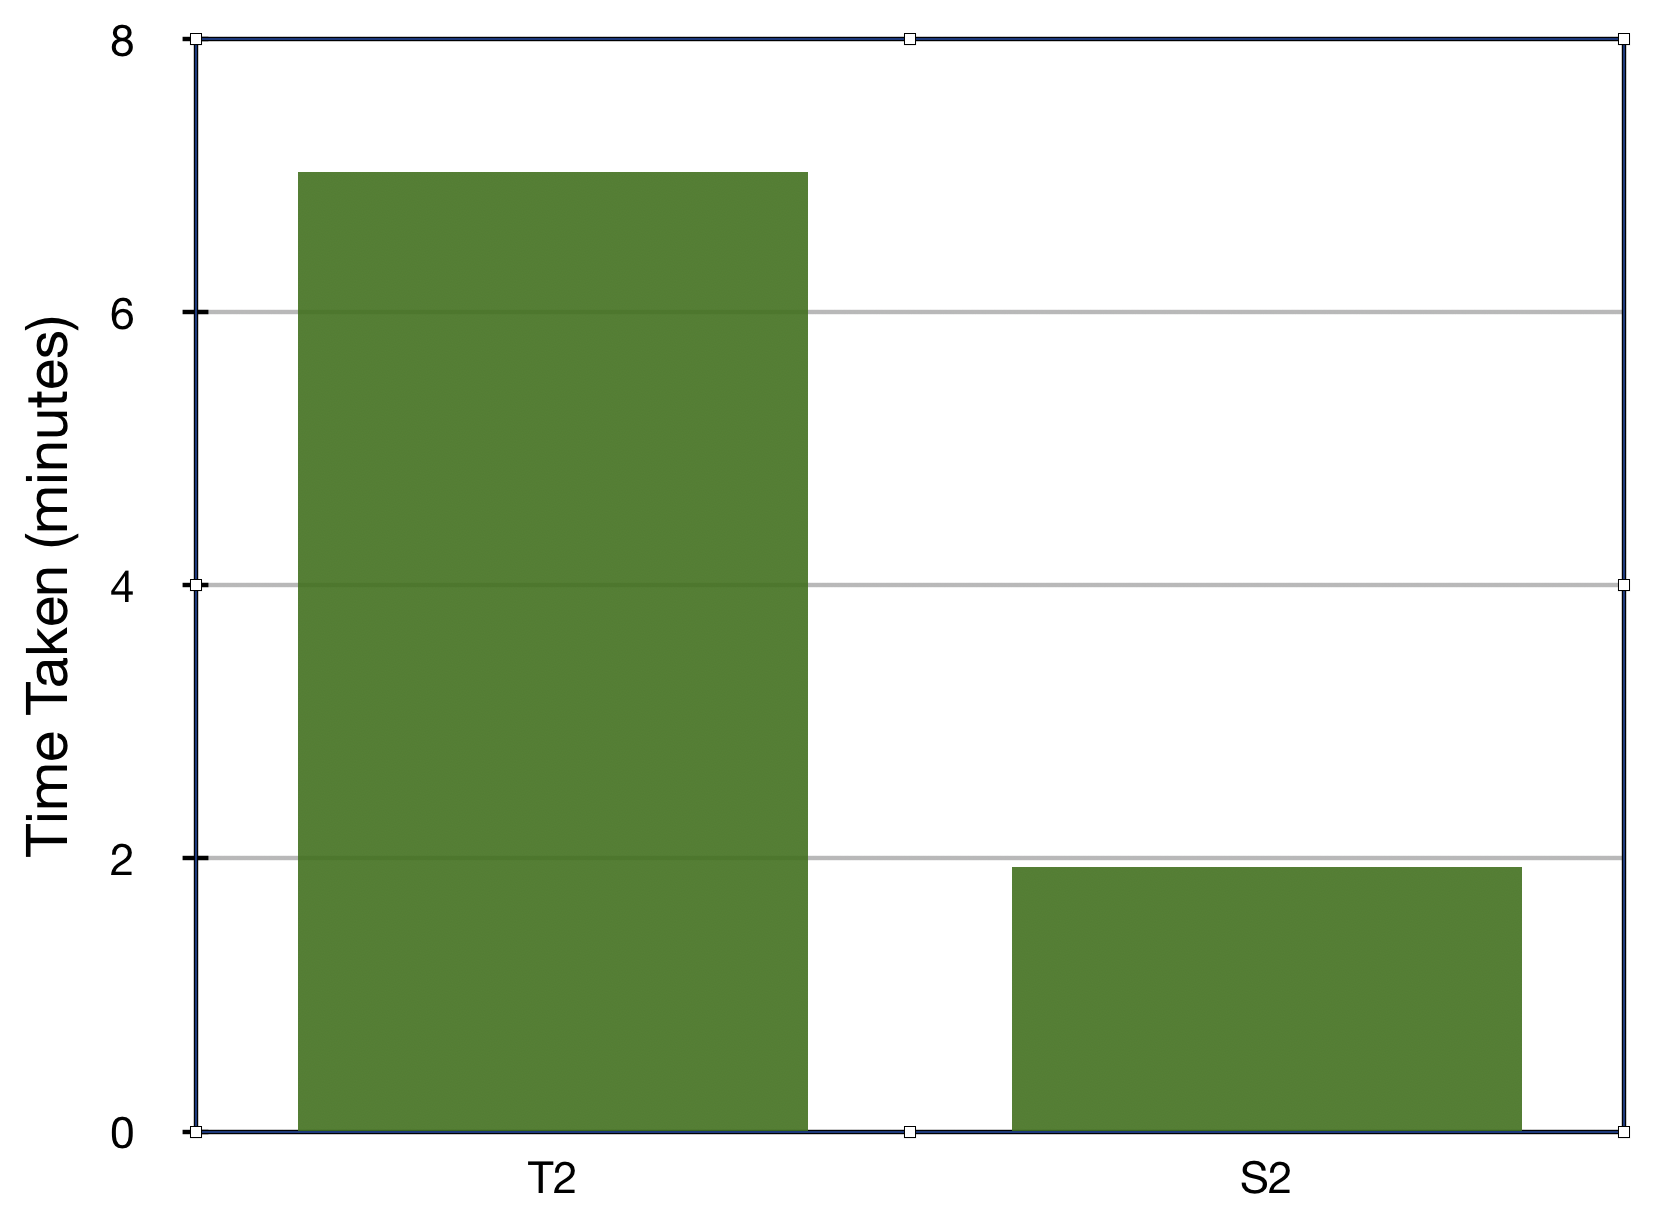
\includegraphics[width=\linewidth]{figs/time.png}
   \caption{Time taken comparison}
   \label{fig:tri_loss}
  \end{subfigure}
    \hfill
    \caption{Comparison of the two best implementations.}
    \label{fig:siatrainloss3}
\end{figure}


\begin{figure}[h]
  \centering
  \begin{subfigure}[b]{0.48\linewidth}
   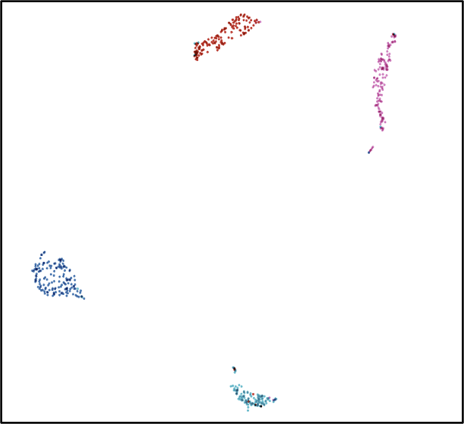
\includegraphics[width=\linewidth]{figs/umab_visualS2.png}
   \caption{Xception + Siamese (S2)}
   \label{fig:tri_loss}
  \end{subfigure}
  \hfill
   \begin{subfigure}[b]{0.48\linewidth}
  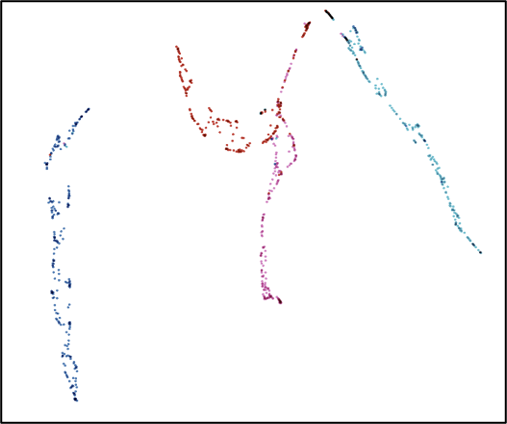
\includegraphics[width=\linewidth]{figs/umab_visualT2.png}
  \caption{Siamese all(T2)}
  \label{fig:con_loss}
  \end{subfigure}
    \hfill
    \caption{visualization of embedded test data projected to 2D space with UMAP using  https://projector.tensorflow.org/.}
    \label{fig:2Dprojection}
\end{figure}

We tried to visualize the comparison of the three implementations of the transfer learning, the three implementations of thesiamese network, and the  two best implementations of both with regards of accuracy and time using a bar graph on figures \ref{fig:siatrainloss1} \ref{fig:siatrainloss2} and \ref{fig:siatrainloss3} respectively.

Furthermore, we can also try to compute the similarity between image pairs, as shown in figure \ref{fig:similarity}. Note that the smaller distance between the two images means they are more similar to each other. For example, in the figure, the distance between the first pair is 0.12, and it turns out that they belong to the same class Slippers. As for the second pair, the class of left image is Slippers and the class of right image is Sandals. The distance between them is 0.56, which is much larger than the first pair, as we expected. 

\begin{figure}[h]
  \centering
  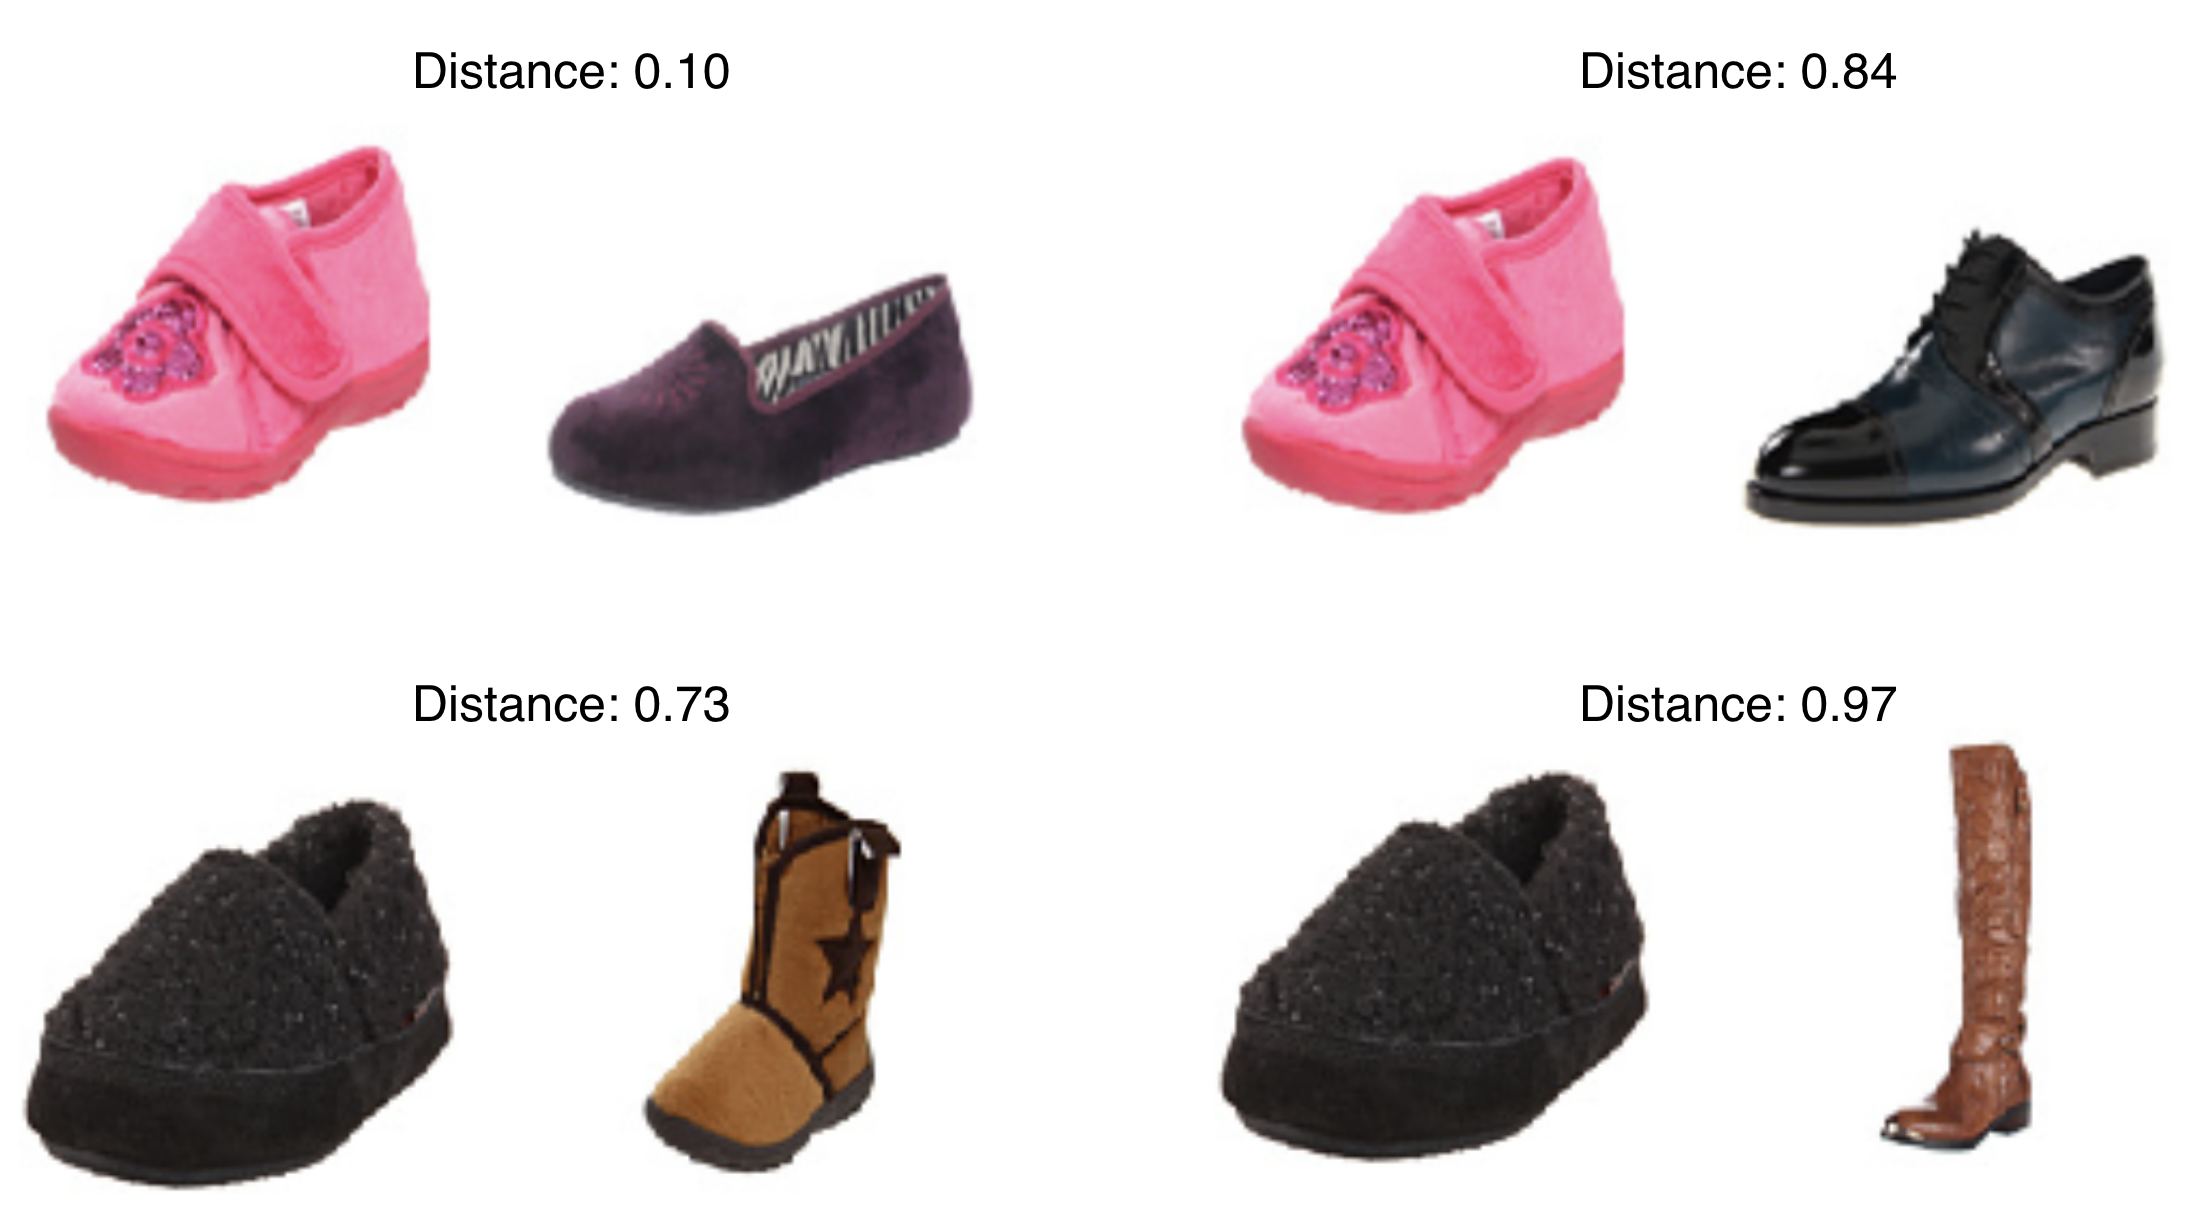
\includegraphics[width=\linewidth]{figs/similarity.png}
  \caption{Examples of calculating the similarity of image pairs.}
  \label{fig:similarity}
\end{figure}


